\documentclass[tikz, border=5pt]{standalone}
\usepackage[utf8]{inputenc}
\usepackage{tikz}
\usetikzlibrary{arrows.meta} % Necesario para >=Stealth

\begin{document}
    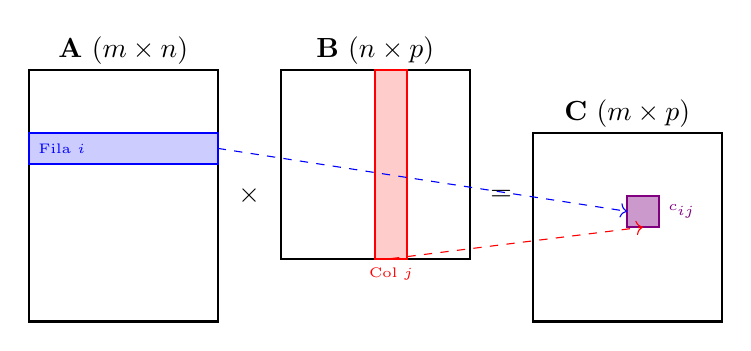
\begin{tikzpicture}[scale=0.8]
        % Matriz A
        \draw[thick] (0,0) rectangle (3,4);
        \node at (1.5, 4.3) {$\mathbf{A} \ (m \times n)$};
        % Fila i resaltada
        \fill[blue!20] (0, 2.5) rectangle (3, 3);
        \draw[thick, blue] (0, 2.5) rectangle (3, 3);
        \node[blue, right] at (0, 2.75) {\tiny Fila $i$};
        
        % Signo multiplicacion
        \node at (3.5, 2) {$\times$};
        
        % Matriz B
        \draw[thick] (4,1) rectangle (7,4); % (n x p) -> ponemos algo cuadrado visualmente
        \node at (5.5, 4.3) {$\mathbf{B} \ (n \times p)$};
        % Columna j resaltada
        \fill[red!20] (5.5, 1) rectangle (6, 4);
        \draw[thick, red] (5.5, 1) rectangle (6, 4);
        \node[red, below] at (5.75, 1) {\tiny Col $j$};
        
        % Signo igual
        \node at (7.5, 2) {$=$};
        
        % Matriz C
        \draw[thick] (8,0) rectangle (11,3); % (m x p)
        \node at (9.5, 3.3) {$\mathbf{C} \ (m \times p)$};
        % Celda ij resultante
        \fill[violet!40] (9.5, 1.5) rectangle (10, 2); % intersección visual relativa
        \draw[thick, violet] (9.5, 1.5) rectangle (10, 2);
        \node[violet, right] at (10, 1.75) {\tiny $c_{ij}$};
        
        % Flechas de flujo
        \draw[->, dashed, blue] (3, 2.75) -- (9.5, 1.75);
        \draw[->, dashed, red] (5.75, 1) -- (9.75, 1.5);
        
    \end{tikzpicture}
\end{document}
